\chapter{Konstruktion von Spielen ausgerichtet auf die User Experience}
\label{Kapitel:uxInSpielen}
%Dieses Kapitel beschäftigt sich mit der Erstellung eines Kriterienkataloges zur Evalution der User Experience in Videospielen. Die zur Evaluation herangezogenen Kriterien, zur Bewertung der User Experience in einem Videospiel, stammen dabei aus verschiedenster Fachliteratur.


In diesem Kapitel wird ein Kriterienkatalog für eine Evaluation der User Experience erstellt. Die zur Evaluation herangezogenen Kriterien, zur Bewertung der User Experience in einem Videospiel, werden durch verschiedenster Fachliteratur gestützt. Abschließend wird zu den einzelnen Kriterien eine Evaluation erarbeitet, mit der die User Experience einzelner Videospiele bewertet werden kann.

%
%
%
%
%Er wird zusätzlich mit einer Auflistung von User Experience Elementen aus diversen Quellen verglichen. Für die gefestigten Kriterien wird eine Evaluation erarbeitet.
%
%
%
%Abschließend wird zu den einzeln kritereien eine evaluation erarbeitet mit dem einzelne videospiel bewertet werden können. 

%Um Spiele auf die User Experience auszurichten, wird ein Kriterien Katalog erstellt. Die aufgestellten   Kriterien werden in Verbindung mit weiteren Elemente der User Experience verknüpft. Für diese Kriterien wird ein Evaluation erarbeitet.







%\section{Auflistung aller Kriterien} 
%%\label{sec:}
%
%
%\begin{description}
%
%\item[Marke/Identität] bei Spielen auch die Erwartung an ein bestimmtes Genre
%
%\item[Ästhetik] 
%
%
%
%Schönheit, Landschaften
%
%\item[Usability] Gilt nicht für die Spiel Logik
%Das erste Kriterium ist die Effektivität
% und bezieht sich darauf, wie genau und vollständig ein Benutzer eine Aufgabe vollenden kann. 
% 
%Das zweite Kriterium ist die Effizienz, es gibt an mit wie viel Aufwand eine Aufgabe im Hinblick auf Genauigkeit und Vollständigkeit fertiggestellt werden kann. 
%
%Das letzte Kriterium greift die Zufriedenheit des Anwenders auf.
%
%
%
%\item[Personalisierungs-/Anpassungsmöglichkeit]
%
%
%
%\item[Inhalt \& Funktionsumfang]
%
%
%\item[Heursitik]
%Ist die Nutzeroberfläche aufgeräumt und leicht verständlich?
%
%Ist die Terminologie an den Benutzer angepasst?
%
%Wird das Gedächtnis des Nutzers nicht zu stark beansprucht?
%
%Ist das System konsistent?
%
%Erhält der Nutzer direktes Feedback durch das System?
%
%Kann das System unkompliziert beendet werden?
%
%Kann ein Nutzer Shortcuts verwenden?    
%
%Gibt es aussagekräftige Fehlermeldungen? Wird der Arbeitsablauf durch sie nicht gestört?
%
%Wird Fehlern vorgebeugt?
%
%Sind Hilfetext und weitere Begleittexte vorhanden?
%
%
%
%\item[Emotionsauslöser]
%
%\begin{itemize}
%\item Lernerfolg
%\item Empathie
%\item Soziale Interaktion 
%\item Herausforderung 
%\item Errungenschaften 
%\item Audio 
%\item Spezial Effekte 
%\item Schönheit 
%\item Landschaftstypen 
%\item Neuheiten 
%\item Urängste 
%\item Sexuelle Signale 
%\end{itemize}
%
%\item[Schwierigkeitsgrad]
%\begin{itemize}
%\item Tiefgang
%\item Zugänglichkeit führt zu  Verfügbarkeit
%\item Neuerfindung
%\item Flexible Herausforderungen
%
%\end{itemize}
%
%\item[Story]
%
%\end{description}


\section{Kriterienkatalog}
\label{Abschnitt:MyKriterienKatalog} 

In den Kapiteln \ref{Kapitel:UX} und \ref{Kapitel:Spielkonzepte} wurden verschiedene Kriterien und Elemente beschrieben, die die User Experience beeinflussen. Die einzelnen Elemente lassen sich teilweise mit den bereits dargestellten Kriterien verbinden oder zu neuen Kriterien zusammenfassen. So lässt sich ein Kriterienkatalog erstellen, mit dem die User Experience eines Videospiels ermittelt werden kann. \\
Die User Experience beginnt bereits vor dem Erwerb eines Spiels. Dies wurde in Abschnitt \ref{Abschnitt:BegriffsdefinitionUX} erläutert. An dieser Stelle gibt es diverse Einstiegshürden, wie den Kaufpreis, das Produktmarketing und persönliche Vorlieben. Nach der Anschaffung folgt die Verwendung des Spiels. Während des Spielens treten die meisten Situationen auf in denen Emotionen ausgelöst werden können. Daher zielt auf diesen Bereich ein Großteil der Kriterien des Kapitels \ref{Kapitel:Spielkonzepte} ab. So sind die Kaufentscheidung und das Spiel selbst die beiden Bereiche in denen die Grundlage für die Erinnerungen liegen und somit die Basis der User Experience. Darüber hinaus gibt es noch weitere Einflüsse, die außerhalb des Spiels wirken. Dazu gehört beispielsweise der Support.  Ein Spieleentwickler hat keinen Einfluss auf den Support, er kann lediglich Anregungen für den Support geben. Daher wird nicht auf alle Einflüsse außerhalb des Spiels eingegangen.




%UX beginnt vor dem Erwerb eines Produktes und geht über dessen Benutzung hinaus.
%Zeitlicher Ablauf: \\
%- Vorwissen \& Erwerb = Einstieg \\
%- Verwendung = USA Kriterien erweitert durch UX + Emotionen, Story \\
%- Erinnerungen = Werden bei der Verwendung erzeugt \\

%Vorwissen \& Erwerb ermöglicht Verwendung \\
%Verwendung erzeugt Erinnerungen \\

%Der Bereich der Verwendung ist der größte und muss aufgeteilt werden. \\

In Abschnitt \ref{Abschnitt:Kriterienkatalog} wurden die grundlegenden Kriterien der User Expierience aufgestellt. Der Erwerb eines Produktes wird durch das Kriterium \textbf{Marke und Identität} beeinflusst. Es bleiben somit vier weitere Kriterien, die auf die Nutzung eines Produktes angewendet werden können. Die \textbf{Ästhetik} spiegelt die Spielatmosphäre wieder. Dies sind die Emotionen, die sich aus den Eindrücken der Spielumgebung zusammensetzen. Die \textbf{Usability} bezieht sich nur auf die direkten Spielereingaben. Die Möglichkeit zur \textbf{Personalisierung} ist in Spielen nur an wenigen Stellen gegeben. Sie bezieht sich hier auf die \textbf{Anpassbarkeit} der Eingabegeräte. Das letzte Kriterium ist der \textbf{Inhalt und Funktionsumfang}. Dieser Punkt beschreibt die Anzahl und den Umfang der Aufgaben, die im Spiel gelöst werden können. In Abschnitt \ref{Abschnitt:Skill} hat sich herausgestellt, dass der Tiefgang, dass heißt der Schwierigkeitsgrad, ein wichtiger Faktor der User Experience in Spielen ist. Dies ist der Punkt der Videospiele von Anwendungssoftware unterscheidet. Denn ein Videospiel muss Aufgaben für einen Spieler generieren und eine Anwendungssoftware hilft einem Benutzer bei der Lösung von Aufgaben. Vor diesem Hintergrund werden die gesamten Kriterien überarbeitet dargestellt: 


%Marke und Identität gehört zum Vorwissen, es bleiben vier Kriterien. 

%Ästhetik - Atmosphäre, Story, Emotion \\
%Usability - Eingaben und Steuerung, nicht die Mechaniken \\
%Inhalt und Funktionsumfang - Story, Tiefgang\\
%Personalisierung - Usability \\

%Herausforderung



\begin{description}
\item[Kaufentscheidung]
%Das Kriterium basiert auf der Marke und Identität. \\
%Bei Software allgemein und auch Videospielen ist die Plattform zu beachten, auf der sie erscheinen. Die Nutzerverteilung ist auf den einzelnen Plattformen z.T. sehr unterschiedlich.\\
%Zusätzlich bringen Spiele in der Regel soziale Interaktionen mit sich, die die Kaufentscheidung beeinflussen. \glqq ...  a colocated social group may provide coaching and critical commentary that substantially adds to the gaming experience \grqq\ \cite[S. 13]{Bernhaupt:2010vi}\\
%Neue Technologien sind eine weitere Quelle für Emotionen, da durch verbesserte Grafik und Interaktionsmöglichkeiten neue Spielerlebnisse entstehen können.



Neue Technologien sind eine Quelle für Emotionen. Durch verbesserte Grafik und Interaktionsmöglichkeiten entstehen neue Spielerlebnisse. Diese können ein Kaufanreiz darstellen. \\
Grundsätzlich ist die Kaufentscheidung abhängig von der Marke und Identität des Produktes. Hat ein Spieler bereits positive Erfahrungen mit einem Spiel aus der selben Reihe oder vom gleichen Entwickler gemacht, wirkt sich dies positiv auf die Kaufentscheidung aus. \\
Auch Meinungsbildung durch soziale Netzwerke kann die Kaufentscheidung beeinflussen \cite[S. 13]{Bernhaupt:2010vi}. \\
Zusätzlich sind Nutzergruppen heterogen über mehrere Plattformen verteilt. Diese Verteilung ist für ein Spiel kaufentscheidend. Besitzt ein Spieler beispielsweise ein iOS Gerät, kann er keine Spiele, die nur für ein anderes Gerät entwickelt wurden, spielen. 



%Vorfeld -  - Einstiegshürde

%UX: Marke/Identität \\
%Emotion: Soziale Interaktion, Neuheit \\

%Anschaffung -> Plattformen -> 

%Einer der wichtigsten Punkte ist die Verfügbarkeit. 
%Ein Spiel, das auf vielen Geräten gespielt werden kann ermöglicht es, dass mehr Spieler ein Spiel spielen können. 
%Daher setzen gerade in der Indie-Szene viele Entwickler auf Plattformunabhängigkeit. Bei großen Spieleherstellern ist dies jedoch wieder etwas anders. So haben alle Spielekonsolen ihre exklusiv Titel.
%Gerade bei Nintendo ist dies sehr ausgeprägt. Dadurch das sie nur Spiele für ihre eigenen Konsolen entwickeln, führt dies dazu, dass Spieler die Konsolen kaufen müssen, die ist aber auch ein etwas umfangreicheres Thema und es müsste tiefer auf die Marketing Aspekte eingegangen werden. Daher ist für die Bewertung zu sagen, je größer die Verfügbarkeit desto besser.

\item[Zugänglichkeit]
Dem Spieler muss ein einfacher Einstieg in ein Spiel möglich sein. So sollten die ersten Level den Spieler nur bedingt fordern, indem flexible Herausforderungen verwendet werden. Bei spielerischen Fehlern sollen Hilfetexte die zu Grunde liegenden Spielmechaniken erläutern. Dieser Faktor wird zum Teil von der Usability abgedeckt. Alle Eingabemöglichkeiten müssen erst vom Spieler erlernt werden. Spieler mit einem höheren Erfahrungslevel fühlen sich durch zu häufige Einblendungen beim Spielen gestört.

%Für Spieler mit einem höheren Erfahrungslevel muss dafür gesorgt sein, dass sie nicht durch zu häufige Einblendungen aus dem Spiel getrieben werden.

% - Einstiegsfreundlichkeit
%UX: Usability

%Schwierigkeitsgrad: Zugänglichkeit, Flexible Herausforderungen \\
%Heuristik: Qualität von Fehlern > Tutorial aussagekräftig, erweiterte Hilfstexte
%Eine große Spielerbasis verbessert das Spielerlebnis. \\
%Spieler finden eher andere Spieler auf ihrem Niveau.\\
%Erlernbarkeit/Zugänglichkeit => keine überladenen Tutorials, die erfahrene Spieler abstoßen.\\

%Im Bezug auf die Grafik: Usability, Control, Skill, Challange


\item[Atmosphäre] - Die audiovisuelle Darstellung eines Spiels steht in Verbindung mit dem Kriterium Ästhetik. Es gibt mehrere Emotionsauslöser, die damit in Verbindung stehen. Es können Personen dargestellt werden, die einen Spieler eine Situation durch Empathie mitfühlen lassen. Auch die Schönheit einer Situation, eines Bildes oder einer Landschaft ruft Emotionen hervor. Zudem nutzen Spezialeffekte, sexuelle Signale und auch die Urängste, Bild und Ton, um auf den Spieler zu wirken.  \\
Die Hintergrundgeschichte eines Spiels ist eng mit diesen Kriterien verbunden. Sie nutzt und erzeugt die Atmosphäre eines Spiels gleichermaßen. \\
Durch die Atmosphäre wird ein Nutzer in eine Spielwelt eingebunden. Je dichter die Atmosphäre ist, umso stärker kann sich der Nutzer in sie hineinversetzten. Er kann sich somit auch besser mit einzelnen Charakteren personifizieren. 

%Eine sehr dichte Atmosphäre, die auf einen Spieler wirkt, wird als immersiv beschrieben. Dieses Wort leitet sich aus dem Begriff Immersion ab. 
%\glqq Wenn wir dem fiktiven Filmgeschehen so weit folgen, dass ein Großteil unserer Aufmerksamkeit dabei absorbiert wird, kann man von Immersion in ein fiktionales Gebilde oder auch von fiktionaler Immersion sprechen.\grqq\ (\cite[S. 69]{Voss:2008vi})



%UX: Ästhetik,
%Emotion: Schönheit, Empathie, Audio, Spezial Effekte, Sexuelle Signale, Urängste, Landschaften

%Story

%durch die Atmosphäre wird der spieler tiefer in die Spielwelt eingebunden. sie ist auch ein nicht zu vergessendes Stilmittel, kann aber auch je nach genre ganz anders aufgefasst werden. sie kann aber auch dabei helfen, ein spiel völlig anders darzustellen. nimmt man z.B. ein Sudoku und fügt statt der zahlen 1-9, 9 verschieden farbige steine, wirkt das ganze trotz gleicher Mechanik völlig anders.

\item[Bedienung]
Ein Spiel muss dem Spieler direktes Feedback geben. Verzögerungen in der Anzeige und bei den Eingaben stören den Spielfluss. Der Spieler muss die Möglichkeit haben einfach durch die einzelnen Spielmenüs zu navigieren. Diese Menüs sollten konsistent strukturiert sein, d.h. sie sollten ein wiederkehrendes festes Schema benutzen.

%Direktes Feedback, einfaches Beenden (mit speichern usw.), anpassbare eingaben (shortcuts)
%Heuristitk: UI aufgeräumt, Konsitenz

\item[Fortschritt]

Lernerfolg ruft Emotionen hervor. Er zeigt dem Spieler einen persönlichen Fortschritt auf. In die gleiche Kategorie fallen die Errungenschaften des Spielers. Sie sind ein Maßstab an dem erkennbar wird, wie lange und mit welcher Intensität ein Spieler ein Spiel gespielt hat. Beide helfen dabei den Spieler auf längere Zeit zu motivieren das selbe Spiel zu spielen.

%Emotion: Lernerfolg
%Schwierigkeitsgrad: Errungenschaften


%Zu Progress gehört zum Beispiel ein Levelsystem, sowie Achievments. Denn der Spieler soll sehen, wie weit er bereits fortgeschritten ist. Zudem soll es motivieren, da dem spieler die ganze Zeit vor Augen gehalten werden soll, wie weit er ist und was er noch tun muss um das nächste lvl zu erreichen oder den nächsten Punkt zu bekommen. Dies kann z.B. auch durch besser werdende Items erzielt werden. Dadurch kann im besten bzw. schlimmsten Fall sogar eine so genannte Suchtspirale entstehen. "Nur noch 3 punkte bis zum nächsten lvl?! Lvl up! Ui jetzt noch einmal 5 das mach ich auch eben noch"


\item[Tiefgang]
%\label{sec:}
Der Tiefgang steht in der Verbindung mit dem Schwierigkeitsgrad eines Spieles. Je mehr Tiefgang ein Spiel bietet, desto länger muss ein Spieler trainieren diesen Tiefgang zu erreichen. Somit ist es neben dem Schwierigkeitsgrad ein Faktor für den Inhalt und Funktionsumfang eines Spiels. Es gibt kleine kurzweilige Spiele mit wenig Tiefgang und umfangreiche Strategiespiele mit viel Tiefgang. 

%UX: Inhalt und Funktionsumfang

%Schwierigkeitsgrad: Herausforderung>>Tiefgang


%Der Umfang eines Spiels beinhaltet vieles zum einen kann dazu die Geschichte gehören zum anderen aber auch die verschiedenen Spiel Elemente. auch beim umfang gibt es eine wie in §x beschrieben eine goldene menge damit der spieler nicht erschlagen wird oder nach nur 5 Minuten schon alles gesehen hat.

%Heuristik: Gedächtnis nicht zu stark beansprucht

\item[Soziale Interaktion]
%\label{sec:}
Mitspieler und selbst Beobachter verändern das Spielerlebnis eines Spielers. Soziale Interaktionen können in einem Spiel gefördert werden. So kann ein Spiel einen Mehrspielermodus besitzen. In einem Mehrspielermodus ist es möglich mit oder gegen andere Menschen zu spielen. \\
Es gibt Spiele die ohne soziale Interaktion nicht möglich sind. Gerade im Bereich der Location-based Games werden häufig mehrere Akteure benötigt. Spiele die auf einem ähnlichen Prinzip wie \glqq GeoCaching\grqq\ basieren sind von einer Person nicht spielbar.

%\glqq Observers in a colocated social group may provide coaching and critical commentary that substantially adds to the gaming experience for those who are playing, and over the course of a play session, may in turn become active players. This is a subarea of social play that also deserves consideration in design and evaluation and is included in this chapter.\grqq\ 


%Soziale Aspekte sind ein zweischneidiges Schwert. Spieler legen wert darauf ihre Spielerfahrungen mit anderen zu teilen. Dadurch sind heutzutage völlig neue Kanäle der Kommunikation entstanden. Sieht man sich die Webseite twitch.tv an, gibt es dort eine Vielzahl von Spielern beim spielen zu schauen. durch die sogenannten lets plays verdienen mittlerweile immer mehr Menschen Geld. Auf der anderen Seite gibt es die von so gut wie allen Spielern als nervig empfundenen Facebook anfragen


%\item[Tension Release - Nicht zwingend eigenes Kriterium]

%Wie in Kapitel §x vorgestellt ist Tension Release der Punkt, um den sich der Spielspaß hauptsächlich dreht. 

%\item[Preis]
%\label{sec:}

%Das Thema Preis ist im Rahmen dieser Arbeit eher ein Randthema, daher wird versucht, die wichtigsten Eckpunkte aufzugreifen um einen groben überblick zu erhalten. Es lässt sich aber erkennen, dass Spieler gerne zu free 2 play Titeln tendieren, da man bei kostenlosen Spielen nichts falsch machen kann. Aber seit der Einführung der apps, hat sich generell einiges am Preismodell vieler Spiele geändert. denn durch einen geringeren Einstiegspreis vergrößert sich auch die Verfügbarkeit.(GENAUER ERKLÄREN!)

\end{description}

\section{Verknüpfung der Kriterien mit weiteren UX-Elementen}

In der Abbildung \ref{pic:uxInGamesExtended} wird eine Sammlung von Elementen, durch die die User Expierience in Videospielen beeinflusst wird, dargestellt. Sie gibt einen Überblick darüber, in welchen Arbeiten welche der einzelnen Aspekte aufgegriffen wurden, die einen Einfluss auf die User Experience haben können. Die einzelnen Elemente der Tabelle sind nicht klar von einander getrennt und überschneiden sich \cite[S. 28]{Bernhaupt:2010vi}. Eine Strukturierung ist möglich, indem sie mit den in Abschnitt \ref{Abschnitt:MyKriterienKatalog} aufgestellten Kriterien verbunden werden.  Es ergeben sich vier über einstimmende Kategorien: 

\begin{itemize}
\item Der Schwierigkeitsgrad besteht aus den Kriterien \textbf{Tiefgang} und \textbf{Zugänglichkeit} und wird in der Abbildung durch die Elemente \textit{skill, competence, challange, focus, concentration} beschrieben.
\textit{Emotionen}. Sie sind grafisch nicht direkt mit den jedem Kriterium verbunden, da sie ein Bestandteil jedes Kriteriums sind.
\item Das Kriterium \textbf{Bedienung} wird in der Abbildung durch die Elemente \textit{control, autonomy, freedom, interactivity, controls, usability} beschrieben.
\item Der Spielinhalt besteht aus den Kriterien \textbf{Atmosphäre} und \textbf{Fortschritt} und wird in der Abbildung durch die Elemente \textit{focus, concentration, physical presence, involvement, meaning, curiosity, story, drama, fantasy} beschrieben.
\item Ein Aspekt in der ursprünglichen Darstellung sind die Emotionen (\textit{emotions}). Nach Abschnitt \ref{Abschnitt:AuslöserEmotionen} sind Emotionen mit allen Kriterien verbunden. 
\item Das Kriterium \textbf{Soziale Interaktion} wird direkt im Aspekt \textit{social interaction} wiedergespiegelt.
\item Das Kriterium der \textbf{Kaufentscheidung} ist in der Grafik nicht berücksichtigt, da sich die Elemente der Grafik nur auf den Spielvorgang beziehen. Kriterien außerhalb des Spielvorgangs bleiben unberücksichtigt.
\end{itemize}






\begin{figure}[H]
    \centering 
    %trim=left buttom right top
    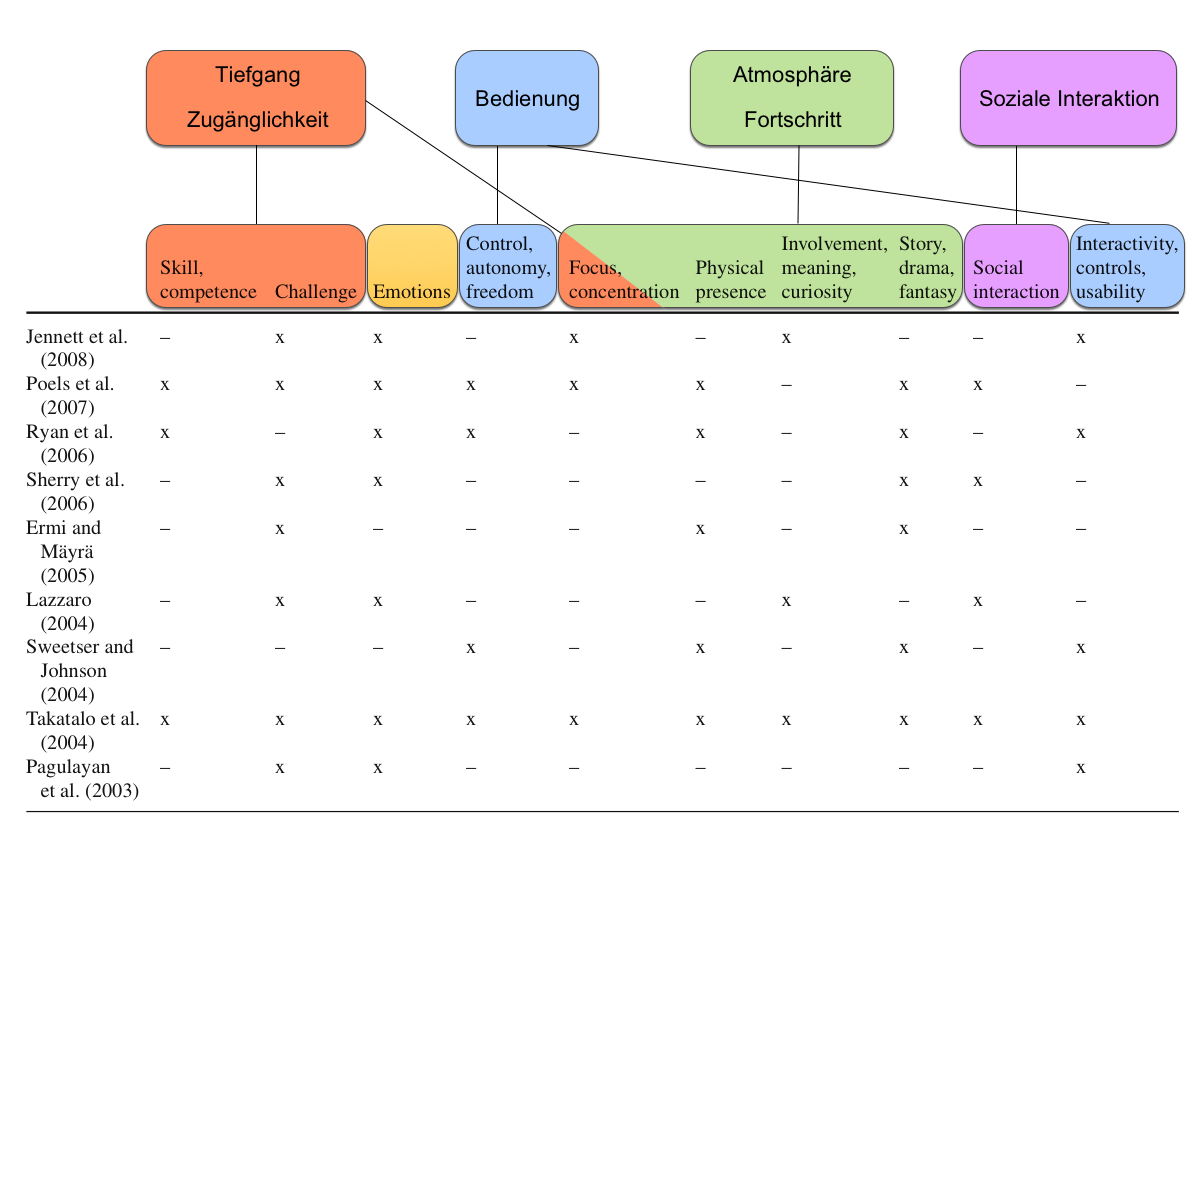
\includegraphics[trim=5 90 3 10,clip,width=1\textwidth]{files/ux/uxInGamesColored}
    \caption{Kriterien der User Experience vgl. \cite[S. 29]{Bernhaupt:2010vi}}
    \label{pic:uxInGamesExtended}
\end{figure}



\pagebreak

\section{User Experience Evaluation}
\label{Abschnitt:AttUXEva}

Parallel zum in Abschnitt \ref{Abschnitt:MethodenEvaluationUX} vorgestellten \textit{AttraktDiff}-Fragebogen lassen sich zu jedem, der in Abschnitt \ref{Abschnitt:MyKriterienKatalog} aufgestellten Kriterien Antonyme zuordnen, mit denen die User Experience bestimmt werden kann. Dafür werden aus jedem Kriterium Schlüsselwörter entnommen, aus denen die Wortpaare abgeleitet wurden.

\begin{description}
\item[Kaufentscheidung:] \  \\
\textit{Schlüsselwörter}: Neue Technologien, Konzepte \\
Sowohl auf der grafischen Ebene als auch auf der spielerischen Ebene  können neue Technologien eingesetzt werden. Ein Spiel kann durch die grafische Präsentation originell oder konventionell wirken. Spielkonzepte erscheinen neuartig oder herkömmlich.
    \begin{itemize}
        \item originell - konventionell %\\
        \item neuartig - herkömmlich
    \end{itemize}
\item[Zugänglichkeit:] \  \\ 
\textit{Schlüsselwörter}: Usability, Schwierigkeitsgrad  \\
Der Einstieg in ein Spiel kann durch die Usability einladend oder zurückweisend sein. Der angeschlossene Spielverlauf kann durch den Schwierigkeitsgrad einfach oder kompliziert sein.
    \begin{itemize}
        \item einfach - kompliziert %\\
        \item einladend - zurückweisend
    \end{itemize}
\item[Atmosphäre:] \  \\
\textit{Schlüsselwörter}: Ästhetik, Handlung, Charaktere \\
Die Ästhetik, in Form der audiovisuellen Darstellung, kann abstoßen oder anziehend sein. Die Handlung eines Spiels kann phantasielos oder kreativ wirken. Die Charaktere eines Spiels können sympathisch oder unsympathisch sein.
    \begin{itemize}
        \item abstoßend - anziehend %\\
        \item phantasielos - kreativ %\\
        \item sympathisch - unsympathisch
    \end{itemize}
    
\item[Bedienung:] \ \\
\textit{Schlüsselwörter}: Spielmenüs, Steuerung bzw. Usability \\
Die Menüs die durch ein Spiel führen, können umständlich oder direkt wirken. Die Steuerung im Spiel kann sich durch Verzögerungen widerspenstig oder handhabbar anfühlen.
    \begin{itemize}
        \item umständlich - direkt%\\
        \item widerspenstig - handhabbar
    \end{itemize}
\item[Fortschritt:] \ \\
\textit{Schlüsselwörter}: Lernerfolg, Errungenschaften \\
Durch Lernerfolg kann sich ein Spiel motivierend oder demotivierend anfühlen. Errungenschaften stellen erreichbare und unerreichbare Ziele dar.
    \begin{itemize}
        \item motivierend demotivierend %\\
        \item erreichbare Ziele - unerreichbare Ziele 
    \end{itemize}
\item[Tiefgang:] \ \\
\textit{Schlüsselwort}: Schwierigkeitsgrad \\
Je nach Schwierigkeitsgrad können Situationen voraussagbar oder unberechenbar sein. Auf der anderen Seite kann eine Aufgabe harmlos oder herausfordernd sein.
    \begin{itemize}
        \item voraussagbar - unberechenbar %\\
        \item harmlos - herausfordernd 
    \end{itemize}
\item[Soziale Interaktion:] \ \\
\textit{Schlüsselwort}: Mitspieler \\
Ein Spiel kann die Spieler voneinander isolieren oder miteinander verbinden.
    \begin{itemize}
        \item isolierend - verbindend
    \end{itemize}
    


\end{description}




%Kaufentscheidung
%	originell konventionell
                            %	innovativ konservativ 
%	neuartig herkömmlich

%Zugänglichkeit 
%	einfach komliziert
%	einladend zurückweisend
                            %	motivierend entmutigend

%Atmosphäre 
%	hässlich schön
                            %	angenehm unangenehm
%	sympathisch unsympathisch
%	phantasielos kreativ
                            %	abstoßend anziehend

%Bedienung 
%	umständlich direkt
%	verwirrend übersichtlich
%	widerspenstig handhabbar

%Fortschritt 
    %motivierend demotivierend
    

%Tiefgang 
%	vorraussagbar unberechenbar
%	harmlos herausfordernd

%Soziale Interaktion 
%	isolierend verbindend
                            %	bringt mich den Leuten näher trennt mich von Leuten
%
%Allgemein 
%	gut schlecht




